\chapter{Размещение базовых станций БШС для обслуживания множества рассредоточенных объектов}\label{ch:ch3}
 
В данной главе будут представлены модели задачи синтеза топологии при развертывании БШС на плоскости для телекоммуникационного покрытия множества рассредоточенных объектов. 

\section{Актуальность внедрения БШС для обслуживания рассредоточенных объектов на месторождении}

Построение современной инфраструктуры передачи информации для обслуживания множества объектов промышленного или гражданского назначения, рассредоточенных на некоторой территории, является актуальной задачей при создании единой систем контроля и управления указанными объектами.  Создание такой инфраструктуры позволяет обеспечить оперативный контроль и управление объектами путем передачи необходимой информации с сенсоров и датчиков объектов в соответствующий внешнее приемное устройство. Для создания подобной инфраструктуры эффективно используются сети широкополосной беспроводной связи, необходимым этапом проектирования которых является решение задачи определения мест размещения базовых станций \cite{VishnevskyBook}.

\fixme{В работе \cite{Mehmood2016} предложен новый протокол сенсорной сети на базе IEEE 802.11 для мониторинга случаев загрязнений углеводородами. В работе \cite{Abbas2021} исследуются различные протоколы сенсорных сетей для мониторинга над газораспределительной сети. Вся сеть разделена на более мелкие, управляемые сегменты, каждый из которых имеет свою базовую станцию для отправки пакетов в центральный пункт управления. В \cite{Bukhari2021} решают задачу размещения мощностей с помощью генетического алгоритма. Авторы занимаются развертыванием устройств распределенных вычислений, серверов, вблизи устройств конечных пользователей. Связующим звеном между конечным пользователем и сервером являются базовые станции.}

В настоящей работе строятся и исследуются две математические модели задач размещения базовых станций, которые применимы на этапе синтеза топологии сети в процессе комплексного проектирования мультимедийных сетей. Предлагается модель для проверки существования допустимого решения при условии выполнении технологических ограничений для предложенной на предыдущих этапах схемы расстановки станций и модель для оптимизационной задачи. Оптимизационная задача состоит в выборе множества станций из заданного набора типов станций с различными характеристиками и их расстановки на избыточном множестве возможных мест размещения. В поставленной задаче рассматривается задача обслуживания объектов, расположение которых задано их координатами на плоскости. Особенностью такой задачи в широком классе задач оптимального размещения мощностей является наличие условия на наличие информационной связи между станциями и внешним приемным устройством (шлюзом), выполнение которого гарантирует поступление всей информации с контролируемых объектов в центр управления. 

Предложена задача оптимального размещения базовых станций, принадлежащая к широкому классу задач размещения мощностей (Resource Allocation Problem). В рамках широкого класса задач размещения мощностей в данных задачах размещения присутствуют специфика на связь между всеми узлами сети. 


% Эффективная политика кэширования контента на границе сети мобильной сотовой связи может улучшить качество услуг для мобильных пользователей и уменьшить перегрузку сети на транзитном рейсе. С другой стороны, виртуализация беспроводной сети становится передовым методом решения проблемы ограниченной пропускной способности сети из-за экспоненциального роста трафика мобильных данных. Кроме того, виртуализация беспроводной сети может принести огромные преимущества, такие как сокращение капитальных затрат (CAPEX) и эксплуатационных расходов (OPEX), а также повышение пропускной способности сети. В этом отношении одним из ключевых требований для признания преимуществ вышеупомянутых двух технологий является наличие применимой структуры распределения ресурсов, которая позволяет развертывать схемы кэширования контента в виртуализированной беспроводной сети. В этом исследовании мы исследуем новую проблему совместного распределения радиоресурсов и кэширования контента, чтобы эффективно использовать блоки радиоресурсов, мощность передачи и доступную кэш-память на базовых станциях (BS). Цель сформулированной проблемы, представленной в этой статье, направлена ​​на минимизацию задержек, с которыми сталкиваются конечные мобильные пользователи операторов мобильных виртуальных сетей (MVNO). Мы показываем, что сформулированная задача является невыпуклой смешанной целочисленной нелинейной задачей (MINLP), которая NP-трудна и просто неразрешима. Поэтому мы применяем алгоритм блочной минимизации верхней границы (BSUM) для решения сформулированной задачи. Численные результаты показывают, что наш метод превосходит существующие базовые схемы распределения ресурсов с приростом производительности до 19% с точки зрения сетевой задержки.}




\section{Математическая модель задачи оптимизации при заданных местах размещения станций.}
Модели задачи оптимизации, которые исследуются в диссертации, предлагается использовать при проектировании БШС на этапе синтеза топологии. После ввода в эксплуатацию сети часто требуется модернизировать, так как любое производство непрерывно развивается. Со временем, телекоммуникационную сеть требует усовершенствование своей инфраструктуры: масштабирование с целью увеличения покрытия сети, демонтаж оборудования, смена протоколов и т.д. Любое изменение приводит к тому, что необходимо провести качество обслуживания сети QoS, надежность и в целом проверить возможно ли обеспечить телекоммуникационное покрытие будущей сети. В данном параграфе будет представлена задача оптимизации при уже заданных размещения базовых станций. В такой постановке возможность сбора такой информации с множества рассредоточенных объектов \fixme{и поиска кратчайшего пути передачи пакетов от множества объектов к шлюзу через множества размещенных станций.}


\subsection{Постановка задачи}

Имеются множество узлов БШС рассредоточенных на плоскости. Все множество можно разбить на две категории:
\begin{itemize}
    \item объекты, с которых необходимо собирать информацию, являются оконечными узлами сети;
    \item станции для сбора и передачи на шлюз данных с объектов, являются промежуточными узлами сети; 
\end{itemize}
Под объектом понимается любое устройство с антенной для передачи пакетов в канале. К ним можно отнести измерительные устройства, шлюзы сенсорных сетей и т.д. В частности, объектами могут быть любые стационарные абонентские устройства сети 802.11n.

Задано множество вершин $A= \left\{ a_i \right\}, i=\overline{0,n}$ на плоскости. Каждая вершина $a_i$ имеет координаты $\left\{ x_i, y_i \right\}$.

Множество $A$ состоит из двух подмножеств:
\begin{itemize}
    \item $A_1$ –- множество вершин, соответствующее объектам; с которых необходимо собирать информацию. 
    \item $A_2$ -- множество мест, где размещены базовые станции. В дальнейшем вершину из $A_2$ будем идентифицировать  не только как место размещения, но и как соответствующую станцию.
\end{itemize}
С вершин $A_1$ необходимо собирать информацию. Каждой вершине $a_i \in A_1$ приписана величина $v_i$ -- максимальный объем информации в единицу времени, который генерирует расположенный на этой вершине объект.  В дальнейшем будем считать, что каждая вершина из $A_1$ является, непосредственно, объектом. В дальнейшем вершинs  $a_i \in A_2$ будем идентифицировать не только как место размещения, но и как соответствующую станцию.

По определению:
$$
A_1 \cup A_2 = \varnothing;
$$

$$
A_1 \cap A_2 = A.
$$

Все вершины пронумерованы так, что:
$$
A_1 = \left\{a_i \right\}, i= \overline{1,n_1};
$$

$$
A_2 = \left\{ a_i  \right\}, i= \overline{n_1+1,n}.
$$

Каждой станции, размещенной на вершине множества $A_2$ приписаны три параметра $s_i = \left\{ \{r_{ij}\}, \{R_{ij}\},\vartheta_i \right\} $, где:

\begin{itemize}
    \item $\{r_{ij}\}$ -- множество радиус телекоммуникационного покрытия станции. Параметр $r_{ij}$ характеризует дальность связи между станцией размещенной в вершине $a_i, a_i \in A_2$ и объектом в вершине $a_j, a_j \in A_1$;
    \item $\{R_{ij}\}$ -- множество радиусов связи станции. Параметр $R_{ij}$ характеризует дальность связи между станциями $s_i$ и $s_j$, $i= \overline{n_1+1,n}, j = \overline{n_1+1,n}, i \neq j$;
    \item $\vartheta_i$ -- объем информации в единицу времени, который может быть получен от объектов, обслуживаемых станцией.
\end{itemize}

Также станция специального вида -- шлюз  $s_0 = \left\{\{R_{0j}\}, \vartheta_0 \right\} $, размещенная на вершине $a_0$ с координатами $\left\{x_0, y_0 \right\}$. Данная станция не имеет телекоммуникационного покрытия и служит для сбора всей информации в сети. По условию задачи величина $\vartheta_0$ больше суммы величин $\vartheta_i$ всех вершин множества $A_1$.

Задано условие, со шлюзом и между собой могут быть связаны только вершины множества $A_2$, то есть только станции.

Требуется проверить, что при заданных наборе и размещении станций на множества $A_2$ вся имеющаяся информация с объектов множества $A_1$ может быть собрана и передана системой станций  до шлюза $s_0$.

\subsection{Модель линейного программирования}
Перед тем как приступить к задаче оптимизации, необходимо подготовить правила составления графа сети, в соответствии с постановкой задачи.

\subsubsection{Граф потока информации}

Составим граф $ H = \left\{A,E \right\} $ для возможного потока информации между вершинами множества $ A = A_1 \cup A_2 $. По определению, каждой вершине $a_i \in A_2 $ соответствует станция $s_i$ со своим набором параметров $s_i = \left\{ \{r_{ij}\}, \{R_{ij}\},\vartheta_i \right\} $.

Матрица смежности $E = \left\{ e_{ij} \right\}$ графа $H$ строится по следующим правилам:

\begin{itemize}
    \item $e_{ij} = 1$, если расстояние между $i$-ым объектом вершины $a_i \in A_1$ и $j$-ой станцией, размещенной на вершине $a_j \in A_2$ не более радиуса покрытия для станции соответствующего этой вершине типа; 
    \item $e_{ij} = 1$, если расстояние между $i$-ой станцией на вершине $a_i \in A_2$ и $j$-ой станцией на вершине $a_j \in A_2$, не более минимального из радиусов связей этих станций;
    \item $e_{i0} = 1$, если расстояние от вершины $a_i \in A_2$ до шлюза не более минимального из радиусов связей станции и шлюза;
    \item $e_{ij} = 0$, во всех остальных случаях.
\end{itemize}

\subsubsection{Формулировка в виде задачи линейного программирования}
С помощью полученного графа смежность $H$, необходимо подготовить условия ограничения для величины потока в каналах.

Введем переменные $x_{ij} \geqslant 0$, определяющее количество информации, передаваемой в единицу времени по дуге $e_{ij}$ графа $H$.

Каждый объект множества $A_1$ генерирует пакеты объемом $\vartheta_i$ в единицу времени. Для канала $e_{ij}, i = \overline{1,n_1}, j = \overline{n_1+1,n}$ величина потока равна весу $\vartheta_i$:

\begin{equation}\label{eq:part2_1.1}
    \sum_{a_j \in \Gamma^+(a_i)} x_{ij} = \vartheta_i, \forall a_i, i=\overline{1, n_1},
\end{equation}
где $\Gamma^+(a_i)$ – множество вершин на графе $H$, в которые входят дуги, исходящие из вершины $a_i$. 

Для каждой вершины $a_i,  a_i \in A_2$ необходимо обеспечить выполнения условия баланса между потоком входящем в эту вершину от объектов множества $A_1$, а также других станций множества $A_2$ и выходящего потока из данной вершины. 

Сумма входящих и выходящих потоков для любой вершины $a_i$  множества $A_2$ должна быть равна нулю:

\begin{equation}\label{eq:part2_1.2}
    \sum_{a_j \in \Gamma_1^-(a_i)} x_{ji} + \sum_{a_j \in \Gamma_2^-(a_i)} x_{ji} -  \sum_{a_j \in \Gamma_2^+(a_i)} x_{ij} =0 ,\forall a_i \in A_2. 
\end{equation}

Здесь множество $\Gamma_1^-(a_i)$ – вершины множества $A_1$, из которых выходят дуги, входящие в вершину $a_i$, $\Gamma_2^-(a_i)$ – вершины множества $A_2$, из которых выходят дуги, входящие в  вершину $a_i$, $\Gamma_2^+(a_i)$ – вершины множества $A_2$, в которые входят дуги, исходящие из вершины $a_i$.


Необходимо чтобы на выходе сети собирался весь трафик. Через систему станций на вершинах $a_j, a_j \in A_2$, вся информация от объектов на вершинах $a_i, a_i \in A_1$ поступала  на шлюз $s_0$:

\begin{equation}\label{eq:part2_1.3}
    \sum_{a_j \in \Gamma_2^-(a_0)} x_{j0} =  \sum_{a_i \in A_1} \vartheta_i;
\end{equation}

\fixme{проверить индексы i, g}

Потока объема информации в каналах ограничен сверху. В случае каналов передачи от объектов на вершинах $A_1$ до станций на вершинах $A_2$ поток ограничен объемом сгенерированного трафика на объекте $\vartheta_i$:

% \begin{equation}\label{eq:part2_1.4_1}
%     \sum_{a_j \in \Gamma_2^+(a_i)} x_{ij} \leqslant \vartheta_i, \forall a_i \in A_1.
% \end{equation}

\begin{equation}\label{eq:part2_1.4_1}
    x_{ij} \leqslant \vartheta_i, \forall a_i \in A_1, a_j \in A_2.
\end{equation}

Объем информации выходящий из станции на вершине $a_j, a_j \in A_2$ ограничен пропускной способностью $\vartheta_j$ станции : 

\begin{equation}\label{eq:part2_1.4_2}
    \sum_{a_i \in \Gamma_2^+(a_j)} x_{ji} \leqslant \vartheta_j, \forall a_j \in A_2.
\end{equation}


Если к системе уравнений ограничений \cref{eq:part2_1.1, eq:part2_1.2, eq:part2_1.3, eq:part2_1.4_1, eq:part2_1.4_2} добавить целевую функцию

\begin{equation}
    \label{eq:part2_1.5}
    \sum_{(a_i, a_j) \in A} c_{ij} x_{ij},
\end{equation}

где $c_{ij}$ -- стоимость потока в ребре, тогда данная модель является задачей о потоке минимальной стоимости. Задача о потоке минимальной стоимости играет одну из основных ролей в области оптимизации сетей \cite{Kovacs2015}. Она используется для нахождения минимальной стоимости потока с множества узлов поставок до множества узлов потребителей в направленном графе с ограничениями на пропускную способность и целевой функцией стоимости, зависящей от пути потока в графе. Задача имеет широкой спектр приложений в различных областях: задачах транспортировки, расписания, ресурсного планирования, телекоммуникации, проектировании сетей и маршрутизации \cite{Kovacs2015, Kiraly2012, Jiang2020} \fixme{добавить}.  

Представленная модель является задачей ЛП, которую можно решить с помощью симплекс-метода \cite{Dantzig1963}. Для решения классическим способом задачи ЛП необходимо задавать ориентированный граф. В случае модели \cref{eq:part2_1.1, eq:part2_1.2, eq:part2_1.3, eq:part2_1.4_1, eq:part2_1.4_2}, ребра графа между станциями $s_j$ в точках $A_2$ двунаправленные. Предполагается, что передача информации может идти в обоих направлениях либо от $s_i$ к $s_j$ через ребро $w_{ij}$, либо от $s_j $ к $s_i$ через ребро $w_{ji}$, соответственно, $i= \overline{n_1+1,n}, j= \overline{n_1+1,n}, i \neq j$ (Рисунок \cref{fig:part3_edges_between_stations}).  Данное особенность задачи портит решение, полученное с помощью классического симплекс метода в линейной форме. Допустимым решением в таком случае будет являться сеть, содержащая циклы между узлами $s_i$ и $s_j$. Для получения объективного решения воспользуемся сетевым симплекс методом, чтобы учесть специфику задачи. 

\begin{figure}[h!]
    \centering
     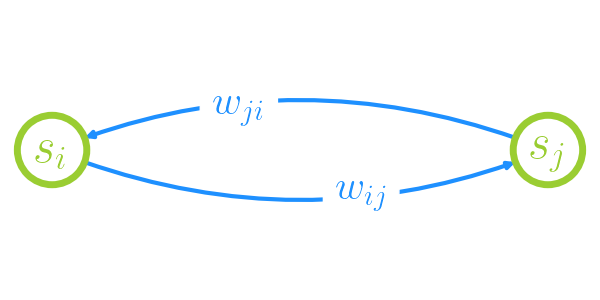
\includegraphics[width=.7\textwidth]{edges_between_stations.png}
  \caption{Направления потоков между станциями.}
  \label{fig:part3_edges_between_stations}
  \end{figure}



С момента публикации Данцигом симплекс-метода \cite{Dantzig1963}, изначально разработанного для задач транспортировки, были получены много новых усовершенствованные моделей, большой обзор метод представлен автором в \cite{Kovacs2015}. Одним из популярных методов решения является сетевой симплекс-метод, которой представляет собой версию хорошо известного симплекс метода ЛП, использующий графовое представление задачи о потоке минимальной стоимости. Метод симплекс-типа применяется для решения задач потока минимальной стоимости. Сетевой симплекс алгоритм с наилучшей стоимостью был разработан Орлином \cite{Orlin1997} в сочетании с древовидной структурой данных Тарьяна \cite{Tarjan1997}. Алгоритм симплекс-метода основана на концепции нахождения минимального остовного дерева. Более подробно алгоритм нахождения решения в виде остовного дерева представлен в работах \cite{Kiraly2012, Kovacs2015, Holzhauser2017, Jiang2020}.

Для нахождения допустимого решения задачи \cref{eq:part2_1.1, eq:part2_1.2, eq:part2_1.3, eq:part2_1.4_1, eq:part2_1.4_2,  eq:part2_1.5} (или доказательства, что допустимого решения не существует) можно найти возможный граф передачи потока информации от объектов до шлюза без учета стоимости потоков. Если ввести единичные стоимости $c_{ij}$ передачи потока $w_{ij}$ по ребру $e_{ij}$ задача \cref{eq:part2_1.1, eq:part2_1.2, eq:part2_1.3, eq:part2_1.4_1, eq:part2_1.4_2,  eq:part2_1.5} будет являться задачей поиска кратчайшего пути от передачи иноформации к шлюзу. \fixme{проверить эту задачу}

% может быть применена стандартная процедура нахождения допустимого решения задачи линейного программирования с вводом искусственных переменных в уравнения \cref{eq:part2_1.1, eq:part2_1.2, eq:part2_1.3, eq:part2_1.4_1, eq:part2_1.4_2} и минимизации состоящей из этих переменных линейной формы. Если значение целевой функции в результате решения задачи окажется больше нуля, то допустимого решения для данного размещения станций не существует, в противном случае полученное решение дает допустимое распределение потоков по каналам связи.

% Далее мы рассмотрим понятие базисных структур в контексте BCMCFPR. В отличие от сетевого симплексного алгоритма для традиционной задачи потока с минимальными затратами (см. [2, стр. 405–407]), нам нужно отказаться от предположения, что подграф, индуцированный базовыми ребрами, не имеет циклов. Вместо этого в основе лежит цикл с ненулевой платой за использование, как это будет подробно показано ниже. 



\fixme{================================================================}

\fixme{После получения, матрицы смежности $H$ необходимо, убедиться, что данный граф является связным. Хотя может это и проверяем в ЛП. Пока так оставить}

\fixme{ПРОВЕРИТЬ Задача о потоке минимальной стоимости}
\fixme{Примем допущение, что интенсивность везде одинакова и равна $\lambda$ . Потом умножить на средий размер пакетов.}
\fixme{Проверить идею кратчайшего остовного дерева. Проверить как считает стоимости}
\fixme{================================================================}



\section{Оптимизационная задача выбора набора размещаемых станций и определения мест их размещения}

\subsection{Постановка задачи.}

Задано множество вершин $A = a_i$, $i=\overline{0,n}$ на плоскости. Каждая вершина $a_i$ имеет координаты $\left\{ x_i, y_i \right\}$.
Множество $A$ состоит из двух подмножеств: 
\begin{itemize}
    \item $A_1$ -- множество вершин, с которых необходимо собирать информацию. Каждой вершине $a_i$ приписана   величина $v_i$ -- максимальный объем информации, снимаемой с объекта, расположенного на этой вершине;
    \item $A_2$ -- множество возможных мест размещения базовых станций. 
\end{itemize}

По определению

$$
A_1 \cup A_2 = A;
$$

$$
A_1 \cap A_2 = \varnothing.
$$

Все вершины пронумерованы так, что:

$$
A_1 = \left\{a_i \right\}, i= \overline{1,n_1};
$$

$$
A_2 = \left\{ a_i  \right\}, i= \overline{n_1+1,n}.
$$


Задано множество типов базовых станций $S = \{s_j$\}, $j=\overline{1,m}$, которые необходимо разместить на множестве точек $A_2$.

Каждой станции приписаны четыре параметра $s_j = \left\{\{r_{ji}\}, \{R_{ji}\}, \vartheta_j, c_j \right\}$, где: 
\begin{itemize}
    \item $\{r_{ji}\}$ -- множество радиусов покрытия. Параметр $r_{ji}$ характеризует телекоммуникационную связь \fixme{доделать} . связи для обеспечения соединения между $j$-ой станцией и объектом, размещенный в координате $a_i$, $j= \overline{n_1+1,n}$, $i= \overline{1,n_1}$. Данный параметр характеризует радиус покрытия станции ;
    \item $R_{ji}$ -- радиус связи между $j$-ой и $i$-ой станциями. Параметр характеризует максимальную дальность связи $j$-ой станции, обеспечивающее заданное качество соединения с $i$-ой станцией, $j= \overline{n_1+1,n}$, $i= \overline{n_1+1,n}$, $j \neq i$;
    \item $\vartheta_j$ -- пропускная способность;
    \item $c_j$ -- стоимость.
\end{itemize}

% максимальный объем информации в единицу времени, который может быть получен от объектов, обслуживаемых данной станцией

Задана станция специального вида (шлюз) $s_0 = \left\{ r_0, \{R_{0j}\}, \vartheta_0, c_0 \right\}$ с координатами $\left\{x_0, y_0 \right\}$. Шлюз уже имеет свое расположение, стоимость размещения $c_0 = 0$. Для шлюз задан параметр радиус связи $\{R_{0j}\}, j = \overline{n_1+1,n}$ для соединения с размещаемыми БС. Полагается, что шлюз не имеет соединения напрямую с объектами $r_0 = 0$. Также будем считать, что шлюз $s_0$ позволяет собрать данные со всех объектов, размещенных в точках $a_i$, $i= \overline{1,n_1}$, в данной постановке задачи пропускная способность равна $\vartheta_0 = \infty$.


Множества вершин $A_1$ будем идентифицировать как размещенные на них объекты. Множества верише $A_2$, на которых будут размещены БС, будем рассматривать, непосредставенно, как сами БС. 

Требуется разместить станции таким образом, чтобы вся информация с объектов на вершинах множества $A_1$ могла быть собрана и передана системой БС, размещенных на выбранных в результате решения задачи в вершинах множества  $A_2$, до шлюза $s_0$ и итоговая стоимость размещения была бы минимальной.

% Вершин и станции будем, соответственно, идентифицировать как объекты или станции на них размещенные.

Задано условие, что информация c вершин множества $A_1$ может передаваться непосредственно только на вершины множества $A_2$, а со шлюзом и между собой могут быть связаны только вершины множества $A_2$.

\subsection{Построение матрицы смежности}

На этапе обследования местности проектировании БШС были отобраны точки, куда возможно расставить БС. Необходимо отметить, что в данной задаче этапа синтеза топологии размещаются не множества имеющихся БС, а выбираются только их типы. Так результатом данного этапа будут набор типов БС и их места размещения.

На каждой вершине $a_i$, $i= \overline{n_1+1,n}$ может разместиться одна из $m$-типов БС. Вместо каждой такой вершины $a_i$ введем $m$ вершин с координатами вершины $\{x_i, y_i \}$, и различными параметрами, соответствующими различным типам станций. Обозначим такую группу вершин, записанных с одинаковыми координатами вместо вершины $a_i$,как $D_i$. Каждой вершине из $D_i$ поставим в соответствие набор параметров только одного типа станции из $S$, т.е. на данной вершине может стоять либо станция приписанного типа либо никакая. Обозначим расширенное множество вершин $A_2$ через $A_2D = \{a_i\}, i = \overline{n_1 + 1,\ n \cdot m}$.

Составим граф $H=\left\{AD,E\right\}$, описывающий сеть для передачи потока информации между вершинами расширенного множества $AD=A_1 \cup A_2D$ и шлюзом.
Матрица смежности $E = \{e_{ij} \}$ графа $H$, где каждое ребро $e_{ij}$ определяет возможность передачи информации между вершинами, строится по следующим правилам. \fixme{проверить индексы для ребра между устройством и станцией.}

\begin{itemize}
    \item $e_{ij} = 1$, если расстояние между $i$-ой вершиной ($a_i \in A_1$) и $j$-ой вершиной ($a_j \in A_2D$) не более радиуса покрытия $r_{ji}$, приписанного этой вершине;
    \item $e_{ij} = 1$, если вершины $a_i$ и $a_j$ принадлежат разным множествам $D_i$ и $D_j$ и расстояние между ними не больше минимального из радиусов связи $\min\{R_{ij}, R_{ji}\}$, приписанных данным вершинам;
    \item $e_{i0} = 1$ ($a_i \in A_2D$), если расстояние от вершины до шлюза не больше минимального радиуса связей $\min\{R_{i0}, R_{0i}\}$;
    \item $e_{ij} = 0$, во всех остальных случаях.
\end{itemize}

\subsection{Математическая модель частично целочисленного линейного программирования}

С помощью полученного графа потока, опишем ограничения для задачи частично целочисленного линейного программирования (ЧЦЛП).

Введем булевы переменную $z_{ij} = \{0, 1\}, i = \overline{1,n_1}, j = \overline{n_1+1, \ n \cdot m}$.


Все объекты, размещенные на вершинах $A_1$, оснащены антеннами для передачи сигнала в беспроводной среде. Каждая объект одновременно может поддерживать соединение только с одной БС. Данной условие можно записать в виде ограничения равенства \cref{eq:part3_only_1_link_from_device}

% Распишем условия для нашей задачи.
% Величина суммарного потока, который выходит с вершины $a_i$ равен весу $\vartheta_i$ \cref{eq:part2_1.5}

\begin{equation}\label{eq:part3_only_1_link_from_device}
    \sum_{a_j \in \Gamma_2^+(a_i)} z_{ij} = 1, \forall a_i, i =\overline{1, n_1},
\end{equation} 
где $\Gamma^+(a_i)$ -- множество вершин на графе $H$, в которые входят дуги, исходящие из вершины $a_i$.

Введем потоковые переменные $x_{ij} \in \mathbb{R}^+$.

Потоки информации объектов с вершин $A_1$ должны поступать на станции. Также на станции может поступать потоки с других станций. Необходимо, чтобы сумма входящих и выходящих потоков для любой $i$-ой вершины множества $A_2D$ был равен нулю \cref{eq:part3_sta_io_flows} \fixme{проверить индексы}
\begin{equation}\label{eq:part3_sta_io_flows} 
    \sum_{a_j \in \Gamma_1^-(a_i)} z_{ij} \cdot \vartheta_i + \sum_{a_j \in \Gamma_2^-(a_i)} x_{ji} -  \sum_{a_j \in \Gamma_2^+(a_i)} x_{ij} =0 ,\forall a_i \in A_2. 
\end{equation} 
Здесь множество $\Gamma_1^-(a_i)$ -- вершины множества $A_1$, из которых выходят дуги, входящие в вершину $a_i$, $\Gamma_2^-(a_i)$ -- вершины множества $A_2D$, из которых выходят дуги, входящие в  вершину $a_i$, $\Gamma_2^+(a_i)$ -- вершины множества $A_2D$, в которые входят дуги, исходящие из вершины  $a_i$.

Через систему станций вся информация от объектов  должна поступить на шлюз $s_0$ \cref{eq:part3_device2gateway_flow} 
\begin{equation}\label{eq:part3_device2gateway_flow}
    \sum_{a_j \in \Gamma_2^-(a_0)} x_{j0} = \sum_{a_i \in A_1} \vartheta_i,
\end{equation}
здесь $\Gamma_2^-(a_0)$ –- подмножество вершин множества $A_2D$, дуги которых входят в шлюз $a_0$.

Введем булевы переменные $y_{ij} = \{0,1\}$ для вершин $a_i$, $a_i \in A_2D$, характеризующие наличие соединения между вершинами.
% \begin{itemize}
%     \item $y_i = 1$, если станция стоит на месте $a_i$;
%     \item $y_i = 0$, в противном случае.
% \end{itemize}

% Объем информации, поступающей от вершин множества $A_1$ на вершину $a_i \in A_2D$, ограничен мощностью станции $\vartheta_i$ \cref{eq:part2_1.8}
Поток информации $w_{ij}$ вершин $a_i$ множества $A_2D$ может передаваться только при наличии соединения $y_{ij}$. Также данный поток ограничен пропускной способностью БС $\vartheta_i$ на вершине $a_i$ \cref{eq:part3_flow_link_sta}
\begin{equation}\label{eq:part3_flow_link_sta}
    \sum_{a_j \in \Gamma_2^-(a_i)} x_{ij} \leqslant y_{ij} \cdot \vartheta_i, \forall a_i \in A_2D.
\end{equation}

Каждая станция может иметь только одно соединение для передачи потока информации в единицу времени. Также необходимо обеспечить условие, что в каждом множестве $D_i$ может быть размещено не более одной станции. Оба этих требования можно записать в виде ограничения неравенства \cref{eq:part3_only_1_link_yij}

\begin{equation}\label{eq:part3_only_1_link_yij}
    \sum_{a_j \in \Gamma_2^-(a_i)} y_{ij} \leqslant 1, \forall D_i.
\end{equation}

Целевая функция задачи минимизации стоимости размещения \cref{eq:part3_of_min}

\begin{equation}\label{eq:part3_of_min}
    \sum_{a_i \in A_2D} \sum_{a_j \in \Gamma_2^-(a_i)}c_i \cdot y_{ij} \to min.
\end{equation}

Задача \cref{eq:part3_only_1_link_from_device, eq:part3_sta_io_flows, eq:part3_device2gateway_flow, eq:part3_flow_link_sta, eq:part3_only_1_link_yij, eq:part3_of_min} представляет собой частично целочисленную задачу линейного программирования с $m \cdot |A_2|$ булевыми переменными.

Численный пример решения задачи оптимизации представлен в Приложении \cref{app:milp_place_solution}.

\section{Выводы к главе 3}
В работе рассмотрены задачи размещения базовых станций при проектировании беспроводных широкополосных сетей связи. Предложены формулировки задач в виде   моделей линейного и частично целочисленного линейного программирования как для случая проверки  наличия допустимых решений для вариантов, предложенных проектировщиками, так и для экстремальной задачи отбора множества станций из имеющегося набора типов станций и оптимального размещения станций выбранного множества на избыточном множестве возможных мест размещения. Предложены алгоритмы построения графов информационных потоков, позволившие формализовать задачи в виде соответствующих моделей математического программирования. Приведены результаты вычислительного эксперимента. Результаты исследования по данной главе были опубликованы в \cite{MukhtarovPershinGUBKIN2018_RSCI, MukhtarovPershinVSPU2019_RSCI, MukhtarovPershinMLSD2019works_RSCI, MukhtarovPershinMLSD2019materials_RSCI,MukhtarovPershinGUBKIN2019_RSCI}. 

\FloatBarrier
